Hops-YARN is a drop-in replacement of Apache Hadoop YARN for the Hops
\cite{hops} platform. From a user's perspective there is no difference
between the two implementations and an Apache YARN application can be
scheduled on Hops-YARN without any modification. Although the
interface is the same, there are some key characteristics that
distinguish the two implementations and can be categorized into
architectural, recovery mechanism and load balancing. In the rest of
the section I will present the differences in every category.

\subsection{Architecture}
\label{ssec:hopsyarn_arch}
In Hops we heavily use a MySQL Cluster that was briefly introduced in
Section \ref{sec:ndb}. We store all kinds of metadata spanning from
Hops-YARN to Hops-HDFS, a new distribution of Apache HDFS, and
HopsWorks, a web-based UI front-end to Hops. The fact that everything
is stored in the database leverages the limited amount of information
that can be stored in the JVM heap of a single machine and opens up
great opportunities of improvement and experimentation.

Apache Hadoop uses ZooKeeper to detect failures and elect a new leader.
Since the MySQL Cluster is already in place storing data, we use a
leader election mechanism proposed by Salman Niazi et
al. \cite{Niazi2015} that uses NewSQL databases in a novel way.
The protocol guarantees a single process acting
as a leader at any point of time with performance comparable to
Apache ZooKeeper. Having the database acting as a persistent storage
and as a leader election mechanism, Hops drops ZooKeeper from its
stack releaving the operations team from the burden of maintaining
one extra service.

\subsection{Fault tolerance \& HA}
\label{ssec:hopsyarn_fault_tol_ha}
In Section \ref{sssec:yarn_ha} I have outlined how Apache Hadoop YARN
deals with RM failures and provides a highly available solution. In
Hops-YARN we follow a different path for storing information for
recovery. In YARN, AMs and NMs communicate with the RM through a
heartbeating mechanism. These heartbeats carry information such as
(de)allocation requests, health status, etc Since the database allows
for millions of transaction per second, we store every single RPC that
the RM receives and delete them when the request is handled. Moreover,
every operation that is done on the scheduler state is reflected on a
modification in the database. The main advantage of this approach over
the approach followed by Apache YARN is in terms of recovery
time. It is much faster to read the complete state of the scheduler from the
distributed in-memory database than asking from every NM to re-sync
and send back a list of all running containers. Particularly when
the cluster size grows in the order of thousands of
machines. Moreover, in case of a crash in Apache YARN, the RM
instructs all the AMs and NMs to re-sync and send again any request
that has been sent but not handled. In Hops-YARN, the RM recovers the
unhandled RPCs from the database and replays them.

In terms of HA the architecture of Hops-YARN is basically the same
with an Active/Standby model for the scheduler, although some
improvements have been made for the Standby nodes described in the
following section.

\subsection{Load balancing}
\label{ssec:hops_yarn_load_balance}
Standby is boring! Except for being boring, having a physical machine
idle for most of the time is a waste of resources. Although RM is a
monolith, its architecture is modular. The components of the RM are illustrated in
Figure \ref{fig:yarn_RM_components}. Hops-YARN follows a very original
approach of distributing the \emph{ResourceTrackerService} among the
StandBy RM nodes. The \emph{ResourceTrackerService} is responsible for
handling the RPCs from the NMs (see Section \ref{sssec:rm}). Assume a
cluster with the moderate size of 5000 nodes and the default value of 1
second for the heartbeat interval. That implies that every second the
RM should handle 5000 RPCs just for keeping track the NM status. In
Hops-YARN, the StandBy RMs also run the
ResourceTrackerService. When NMs register with the RM they are
assigned to the least overloaded \emph{ResourceTracker} (RT) -- StandBy
\emph{ResourceManager}. The information received by each
\emph{ResourceTracker} separately is stored in the
database and through the event API of NDB is streamed to the Active
RM to update its view of the cluster. In that case, NDB serves as a
communication channel between the RT and the RM. With that
architecture the load of tracking 5000 nodes is distributed among all
the RMs in the cluster. An overview of Hops-YARN distributed
ResourceManager is illustrated in Figure \ref{fig:hopsyarn_dist_rm}.

\begin{figure}
\centering
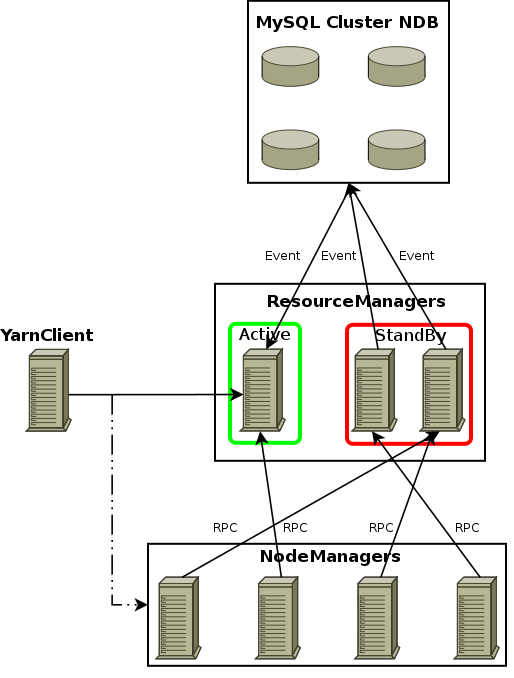
\includegraphics[scale=0.5]{resources/images/Background/hopsyarn_arch_overview.png}
\caption{Hops-YARN distributed RM architecture}
\label{fig:hopsyarn_dist_rm}
\end{figure}